\documentclass[letterpaper, 11pt]{article}
    \usepackage[margin=0.9in]{geometry}
    \usepackage{graphicx, hyperref, enumitem, booktabs}
    \usepackage{cancel, verbatim}
    % rubber: set program xelatex
    \usepackage[calc,linalg,physics,stix]{bccho}

    \usepackage{tocloft}
    \usepackage{etoc}
    \usepackage[margin=1cm]{caption}
    \usepackage[labelformat=simple]{subcaption}
    \usepackage{float}
    % rubber: setlist arguments --shell-escape
    \usepackage{minted}
    \usepackage[linewidth=0pt]{mdframed}

    \definecolor{bg}{rgb}{0.95, 0.95, 0.95}
    \BeforeBeginEnvironment{minted}{\begin{mdframed}[backgroundcolor=bg]}
    \AfterEndEnvironment{minted}{\end{mdframed}}

    % \renewcommand{\thefigure}{\thesection.\arabic{figure}}
    \captionsetup[figure]{labelfont={it,bf}}
    \captionsetup[table]{labelfont={it,bf}}
    \captionsetup[subfigure]{labelfont={it}}
    \renewcommand\thesubfigure{(\alph{subfigure})}

    \newcommand*{\figref}[1]{\textbf{\figurename~\ref{#1}}}
    \newcommand*{\tblref}[1]{\textbf{\tablename~\ref{#1}}}

    \newcommand{\iic}{I$^2$C\xspace}
    \renewcommand{\v}[1]{\vec{#1}}

% Begin document

\begin{document}
\section{Theory}
\subsection{Stereo vision}
We used a pinhole camera model for our Pixy cameras. Under this model, points in 3-D world coordinates are projected onto an imaging plane using homogenous coordinates. In the simplified case when the camera is at the origin pointing in the positive $z$ direction (i.e. the image plane is at $z=1$), we convert from world coordinates $(x, y, z)^T$ to image coorinates $(m, n)^T$ using basic linear algebra. First, we define $\paren{x', y', z'}^T$ as follows:
\begin{align*}
    \pmat{x' \\ y' \\ z'} &= \pmat{f_x & 0 & c_x \\ 0 & f_y & c_t \\ 0 & 0 & 1} \pmat{x \\ y \\ z} \\
    \intertext{The $3\times 3$ matrix is known as the \textbf{camera intrinsic matrix}, $F$, with entries $f_x$ and $f_y$ that represent the scale of conversion between world units and pixel units, and $c_x$ and $c_y$ that are the horizontal and vertical offsets of the image origin in pixels. Since these are all parameters internal to the camera, they are known as intrinsic parameters. Typically, $c_x$ and $c_y$ correspond to half of the width and height of the output image respectively. Then, to convert to image coordinates we simply divide by the $z'$-component:}
    \pmat{m \\ n} &= \pmat{ x' / z' \\ y' / z' }
\end{align*}
Concisely, we can write $\vec{w}_h \equiv F \vec{w}$ where $\vec{w}_h = (m, n)^T$ and $\vec{w} = (x, y, z)^T$, and $\equiv$ represents the process of dividing by the third component. If the camera is located at a point $\vec{p}$ from the origin, we can simply modify this equation to read $\vec{w}_h \equiv F(\vec{w}-\vec{p})$.

The problem with position estimation with one camera is that this perspective projection is not reversible (the input has three degrees of freedom, while the output only has two), so we need some additional source of positional information in order to recover the third degree of freedom. We briefly considered using a single camera (for simplicity) and the observed size of the ball, since linear dimensions should scale with $1/z$ with distance from the camera, while the area should decrease with $1/z^2$. However, we quickly switched to using two cameras because (1) at reasonable distances (even as close as three feet away from the camera), the observed size of the ball was too small (on the order of tens of pixels) that it would have produced unacceptable granularity in our depth measurements; and (2) the image processing of the Pixy camera was noisy and caused the area to fluctuate too much, producing noise in depth that would have been unacceptable for trajectory estimation.

Given image coordinates from two identical cameras with a known translational separation (and to simplify our calculations, no rotation), we can recover the original $z$-component in world coordinates by solving
\begin{align*}
    &\lb{
        \v{w}_{h1} &\equiv F\paren{\v{w}-\v{p}_1} \\
        \v{w}_{h2} &\equiv F\paren{\v{w}-\v{p}_2} \\
    } \\
    \implies &\pmat{m_1 - m_2 \\ n_1 - n_2 \\ z} \equiv F\paren{\v{p}_2 - \v{p_1}} \\
    \intertext{If there is only an $x$-displacement between the two cameras, we can estimate $z$ directly from only the horizontal disparity in the images:}
    \implies &z = \frac{f_x t_x}{m_1 - m_2}
\end{align*}
where $t_x = \paren{\v{p}_{2} - \v{p}_{1}}_x$.

The convention for camera coordinates typically has $z$ along the principal axis of the camera, but since our camera was mounted on the front of the robot, we performed a basic coordinate transform so that $z$ was vertical (normal to the ground):
\begin{align*}
    x\sub{world} &= x\sub{camera} & y\sub{world} &= z\sub{camera} & z\sub{world} &= y\sub{camera}
\end{align*}
For trajectory estimation and prediction, we used only world coordinates to avoid confusion.

It is important to note that the Pixy camera is not an ideal pinhole camera. Critically, it exhibits radial distortion. We attempted correcting for this by calibrating using MATLAB's camera calibration methods (e.g. the \verb|cameraCalibrator| app), but we found little significant improvement in position estimation, and the small position differences from the distorted image and coordinates were sufficient for our purposes.

\subsection{Trajectory estimation and prediction}
Trajectory estimation is the process of performing statistical estimation of kinematic parameters, such as initial position and velocity in all three spatial dimensions, and acceleration in the world $z$-axis. Among our many design iterations, we also estimated the coefficient of restitution from our observed data. We approached trajectory estimation with a linear regression model with various modifications, and then used the estimated kinematic parameters to estimate the time and location of bounces (i.e. perform trajectory prediction). We decided to use regression instead of finite difference methods because we expected our stereo ball tracking data to be rather noisy (finite differences tend to amplify high-frequency noise).

We divided our model of the ball's trajectory into the global $x$, $y$ and $z$ coordinates (relative to the robot, since we simplified our problem by tracking the ball only while the robot was stationary). For the $x$ and $y$ coordinates, we performed simple linear regression over all detected ball positions:
\begin{align*}
    x &\sim \beta_{x0} + \beta_{x1}t & y &\sim \beta_{y0} + \beta_{y1}t
\end{align*}
For the $z$ coordinate, we performed linear regression with quadratic time features:
\begin{align*}
    z &\sim \beta_{z0} + \beta_{z1}t + \beta_{z2}t^2
\end{align*}
$\beta_{x0}$, $\beta_{y0}$ and $\beta_{z0}$ all represent the initial positions (at $t=0$); $\beta_{x1}$, $\beta_{y1}$ and $\beta_{z1}$ all represent the initial velicities (at $t=0$); and $\beta_{z2}$ represents the acceleration due to gravity.

All of these regression models can be written as $\v{Y} \sim \mat{X} \v{\beta}$ where $\mat{X}$ is the $n\times d$ feature matrix: for the $x$ and $y$ coordinates, $\mat{X}$ consists of a column of ones, and a column for $t$; for the $z$ coordinate, $\mat{X}$ consists of a column of ones, a column for $t$, and a column for $t^2$. Then, assuming that $n\ge d$ so that $\mat{X}$ is not rank-deficient, by ordinary least squares (OLS) we have a simple formula for the regression coefficients, $\v{\beta}$:
\[ \hvec{\beta}\sup{OLS} = \paren{ \mat{X}^T\mat{X} }\inv \mat{X}^T \v{Y}. \]

The $z$-coordinate regression model is, however, rather limited: since it represents a pure parabola, it cannot take bouncing into account. To overcome this, we implemented a transform mapping points from after a bounce back onto the original parabola to continue to improve our regression coefficients; this transform was based on the observation that the parabola after a bounce is a scaled version of the original parabola (see \figref{fig:bounce} below).

Specifically, the bounce height and duration are completely determined by the velocity of the ball after the bounce, so if $R$ is the coefficient of restitution (i.e. the ratio between energy after and before a bounce, or equivalently, between the maximum height before and after a bounce), the velocity after the bounce is scaled by $\sqrt{R}$, the height is scaled by $R$, and the duration of the bounce is scaled by $\sqrt{R}$ (since bounce duration is given by $2v\sub{init} - gt\sub{duration}$). Therefore, in order to rescale the data back to the first parabola, we reflect time points $t \mapsto t\sub{bounce} - \paren{t - t\sub{bounce}} / \sqrt{R}$ and scale $z \mapsto z / R$. This is demonstrated in \figref{fig:transform} below.

\begin{figure}[ht]
    \centering
    \begin{subfigure}[t]{0.48\textwidth}
        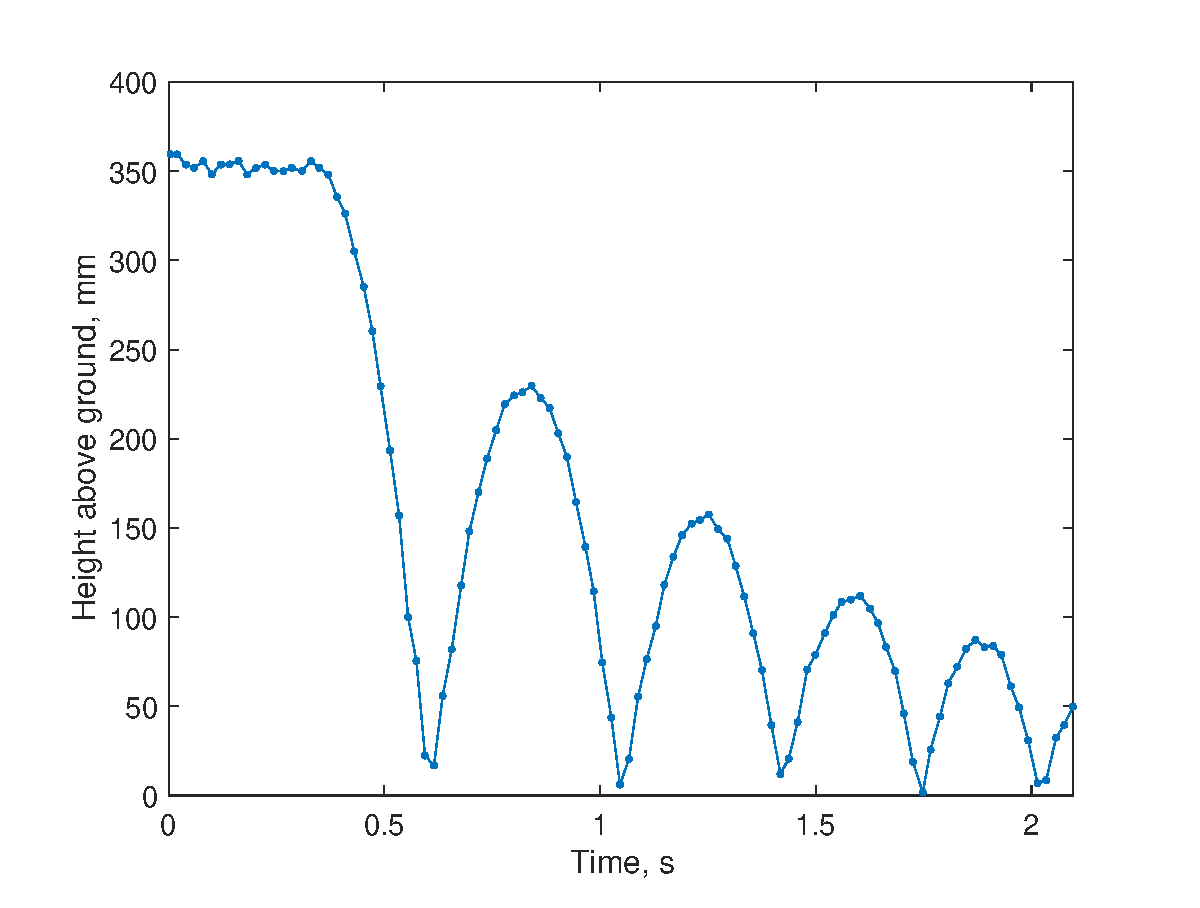
\includegraphics[width=\textwidth]{images/fig_bounce.eps}
        \caption{Plot of ball height over several bounces.}
        \label{fig:bounce}
    \end{subfigure}%
    \begin{subfigure}[t]{0.48\textwidth}
        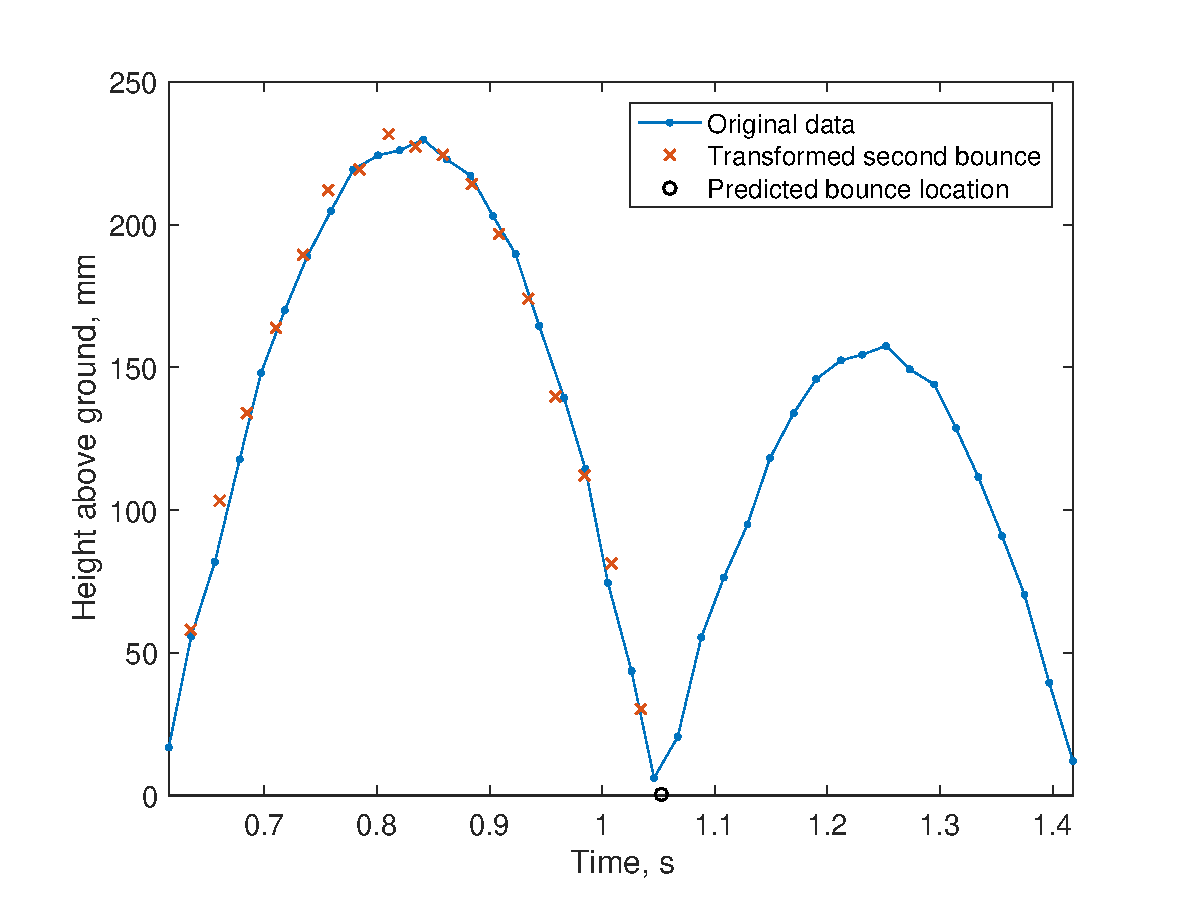
\includegraphics[width=\textwidth]{images/fig_transform.eps}
        \caption{Demonstration of reflection and rescaling transform, using $R = 0.68$.}
        \label{fig:transform}
    \end{subfigure}
    \caption{\textbf{Kinematics of ball-bouncing.}}
\end{figure}

However, this introduces a new free parameter, $R$. We cannot regress for $R$ using linear regression, because the model is no longer linear: $z \sim \paren{\beta_0 + \beta_1 t + \beta_2 t^2} / R$. Thus, we were forced to either hard-code a value for the coefficient of restitution, or attempt to minimize the mean-squared error among a range of $R$ values (since reasonable values of $R$ were between $0.2$ and $0.8$). We initially attempted to implement the latter, but in the late hours of Wednesday night / Thursday morning, something was wrong in our implementation and we decided to hard-code a value of $R$ based on the surface and type of ball we were working with.

\subsection{Omni-drive}
\end{document}
